\documentclass[aspectratio=169,11pt]{beamer}

\usetheme{Madrid}
\usecolortheme{dolphin}
\setbeamertemplate{navigation symbols}{}
\setbeamertemplate{theorems}[numbered]

\usepackage[utf8]{inputenc}
\usepackage[T1]{fontenc}
\usepackage{lmodern}
\usepackage{amsmath,amssymb,amsthm,mathtools}
\usepackage{bm}
\usepackage{booktabs}
\usepackage{graphicx}
\usepackage{listings}
\usepackage{xcolor}

\newcommand{\ones}{\mathbf{1}}
\newcommand{\diag}{\operatorname{diag}}
\newcommand{\KL}{\operatorname{KL}}
\newcommand{\Tset}{\mathcal{T}}
\newcommand{\Piset}{\Pi}
\newtheorem{proposition}{Proposition}

\lstdefinestyle{py}{
  language=Python,
  basicstyle=\ttfamily\scriptsize,
  keywordstyle=\color{blue!70!black},
  commentstyle=\color{green!40!black},
  stringstyle=\color{red!60!black},
  showstringspaces=false,
  frame=single,
  breaklines=true,
  tabsize=2
}

\title{Discrete Diffusion Tutorial}
\subtitle{Forward Noising, Reverse Kernels, and Learning}
\author{}
\date{}

\begin{document}

\begin{frame}
  \titlepage
\end{frame}

\begin{frame}{Roadmap}
\tableofcontents
\end{frame}

\section{Forward Process}

\begin{frame}{State Space and Histograms}
We work on a finite state space $\mathcal X=\{1,\dots,n\}$.

A histogram at time $t$ is
\[
h^t\in\mathbb R_+^n,\qquad \sum_{i=1}^n h_i^t=1.
\]

A forward kernel is row-stochastic:
\[
P\in\mathbb R_+^{n\times n},\qquad P\ones=\ones,
\qquad P_{ij}=\mathbb P(X_{t+1}=j\mid X_t=i).
\]
\end{frame}

\begin{frame}{Forward Dynamics}
\begin{block}{Definition (Forward recursion)}
\[
h^{t+1}=P^\top h^t,\qquad t=0,\dots,T-1.
\]
\end{block}

\begin{proposition}
If $h^0\in\Delta_n$ and $P\ones=\ones$, then each $h^t\in\Delta_n$.
\end{proposition}
\begin{proof}
Non-negativity is immediate since $P\ge 0$. Also
\[
\ones^\top h^{t+1}=\ones^\top P^\top h^t=(P\ones)^\top h^t=\ones^\top h^t=1.
\]
\end{proof}
\end{frame}

\begin{frame}{Examples of Forward Kernels}
\begin{itemize}
\item Local 3-neighbor (random walk style):
\[
P_{ij}=\tfrac13\mathbf 1_{j\in\{i-1,i,i+1\}}
\]
(with boundary convention).
\item Gaussian convolution:
\[
P_{ij}\propto \exp\!\left(-\frac{(i-j)^2}{2\sigma^2}\right),\qquad \sum_j P_{ij}=1.
\]
\item Masking/absorbing (toward a special state $n$):
\[
P_{ii}=1-\varepsilon,\quad P_{in}=\varepsilon,\quad P_{nn}=1.
\]
\end{itemize}
\end{frame}

\section{Backward Kernels}

\begin{frame}{Admissible Reverse Kernels}
Fix two histograms $a,b\in\Delta_n$.

\begin{block}{Definition}
\[
\Tset(a,b)=\{K\ge 0:\ K\ones=\ones,\ K^\top a=b\}.
\]
\end{block}

In diffusion, reverse kernels satisfy
\[
Q^t\in\Tset(h^{t+1},h^t),\qquad t=0,\dots,T-1.
\]
So there are exactly $T$ reverse kernels connecting $t+1\to t$.
\end{frame}

\begin{frame}{Backward Particle Process}
\begin{block}{Definition (Backward chain)}
\[
Y_T\sim h^T,\qquad Y_t\sim Q^t(Y_{t+1},\cdot),\ t=T-1,\dots,0.
\]
\end{block}

\begin{proposition}
If each $Q^t\in\Tset(h^{t+1},h^t)$, then
\[
\mathrm{Law}(Y_t)=h^t\quad\text{for all }t.
\]
\end{proposition}
\begin{proof}
Backward induction:
$\mathrm{Law}(Y_T)=h^T$ by initialization.
If $\mathrm{Law}(Y_{t+1})=h^{t+1}$ then
\[
\mathrm{Law}(Y_t)=(Q^t)^\top h^{t+1}=h^t.
\]
\end{proof}
\end{frame}

\begin{frame}{Bayes Inverse Kernel}
Given forward $P\in\Tset(h^t,h^{t+1})$, define
\[
Q^{\mathrm B,t}_{ij}=\mathbb P(X_t=j\mid X_{t+1}=i).
\]

\begin{proposition}[Bayes formula + matrix form]
For $h^{t+1}_i>0$,
\[
Q^{\mathrm B,t}_{ij}=\frac{h_j^tP_{ji}}{h_i^{t+1}},
\qquad
Q^{\mathrm B,t}=\diag(h^{t+1})^+P^\top\diag(h^t).
\]
Moreover $Q^{\mathrm B,t}\in\Tset(h^{t+1},h^t)$.
\end{proposition}
\end{frame}

\begin{frame}{Couplings and Kernels}
Define coupling polytope:
\[
\Piset(a,b)=\{\pi\ge 0:\ \pi\ones=a,\ \pi^\top\ones=b\}.
\]

\begin{proposition}[Bijection]
\[
\Phi_{a,b}:\Tset(a,b)\to\Piset(a,b),\qquad \Phi_{a,b}(K)=\diag(a)K
\]
is bijective on $\operatorname{supp}(a)$ with inverse
\[
\Phi_{a,b}^{-1}(\pi)=\diag(a)^+\pi.
\]
\end{proposition}

\vspace{0.3em}
Interpretation: learning $Q^t$ is equivalent to learning a coupling $\pi^t$ with fixed marginals.
\end{frame}

\section{Numerics}

\begin{frame}{Numerical Setup}
We use the same setup as the notebook:
\begin{itemize}
\item $n=30$, $T=100$, $N=2500$, $\sigma=0.75$.
\item Initial histogram: 3 spikes at $[0.1,0.6,0.8]\cdot n$ with amplitudes $[1,1.4,0.6]$ (normalized).
\item Forward kernel: Gaussian convolution
\[
P_{ij}\propto \exp\!\left(-\frac{(i-j)^2}{2\sigma^2}\right).
\]
\item Reverse kernels: Bayes inversion
\[
Q^t=\diag(h^{t+1})^+P^\top\diag(h^t).
\]
\end{itemize}
\end{frame}

\begin{frame}{Forward Simulation Results}
\begin{columns}[T]
\begin{column}{0.49\textwidth}
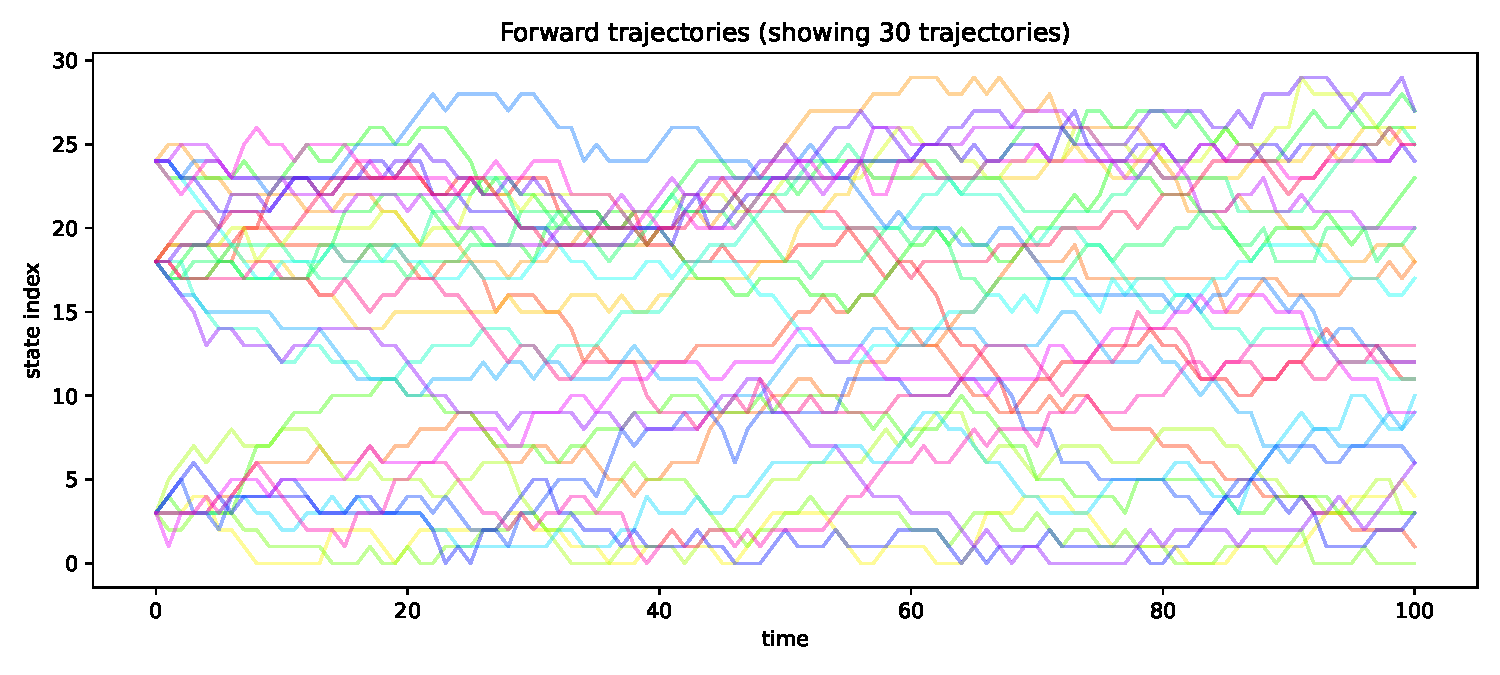
\includegraphics[width=\linewidth]{../tutorial/figures/forward_trajectories.pdf}
\end{column}
\begin{column}{0.49\textwidth}
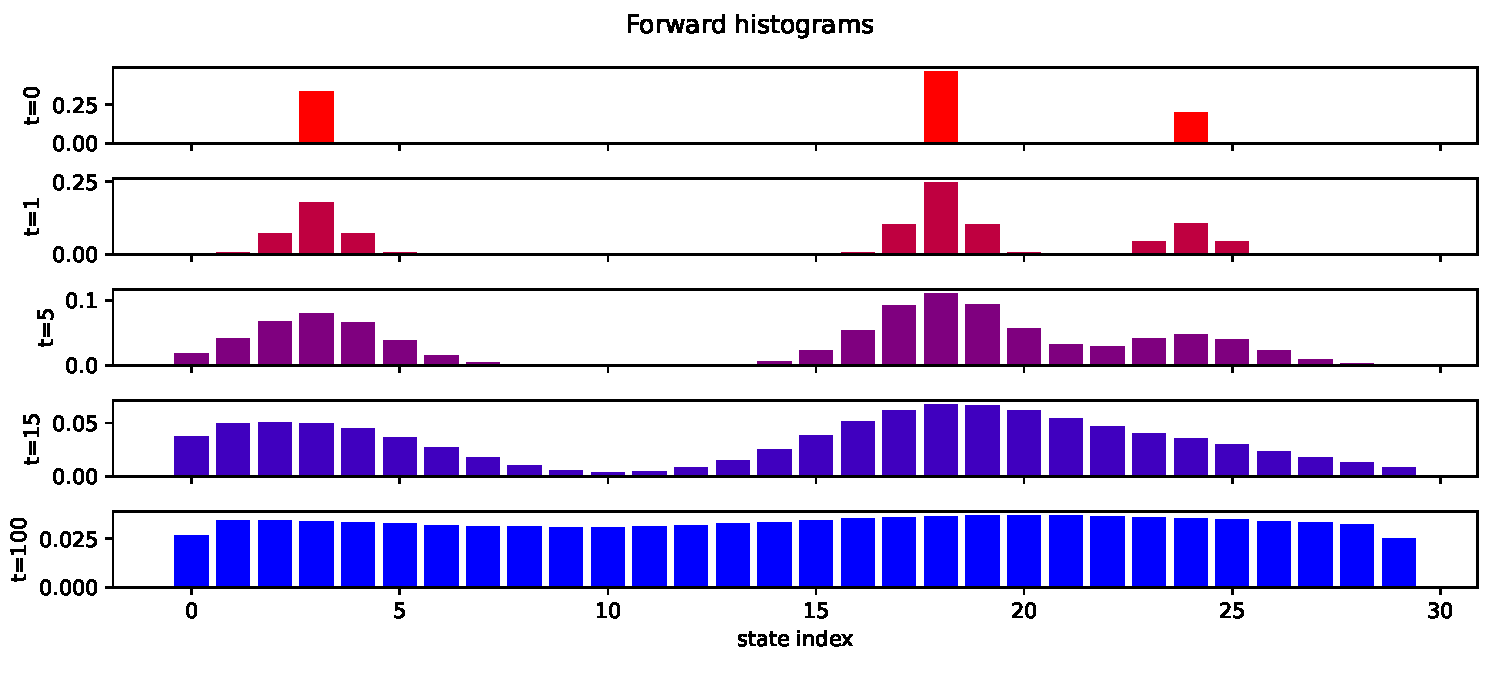
\includegraphics[width=\linewidth]{../tutorial/figures/forward_histograms.pdf}
\end{column}
\end{columns}
\vspace{0.4em}
\small Left: 30 trajectories. Right: snapshots at $t=0,1,5,15,T$.
\end{frame}

\begin{frame}{Backward Simulation Results}
\begin{columns}[T]
\begin{column}{0.49\textwidth}
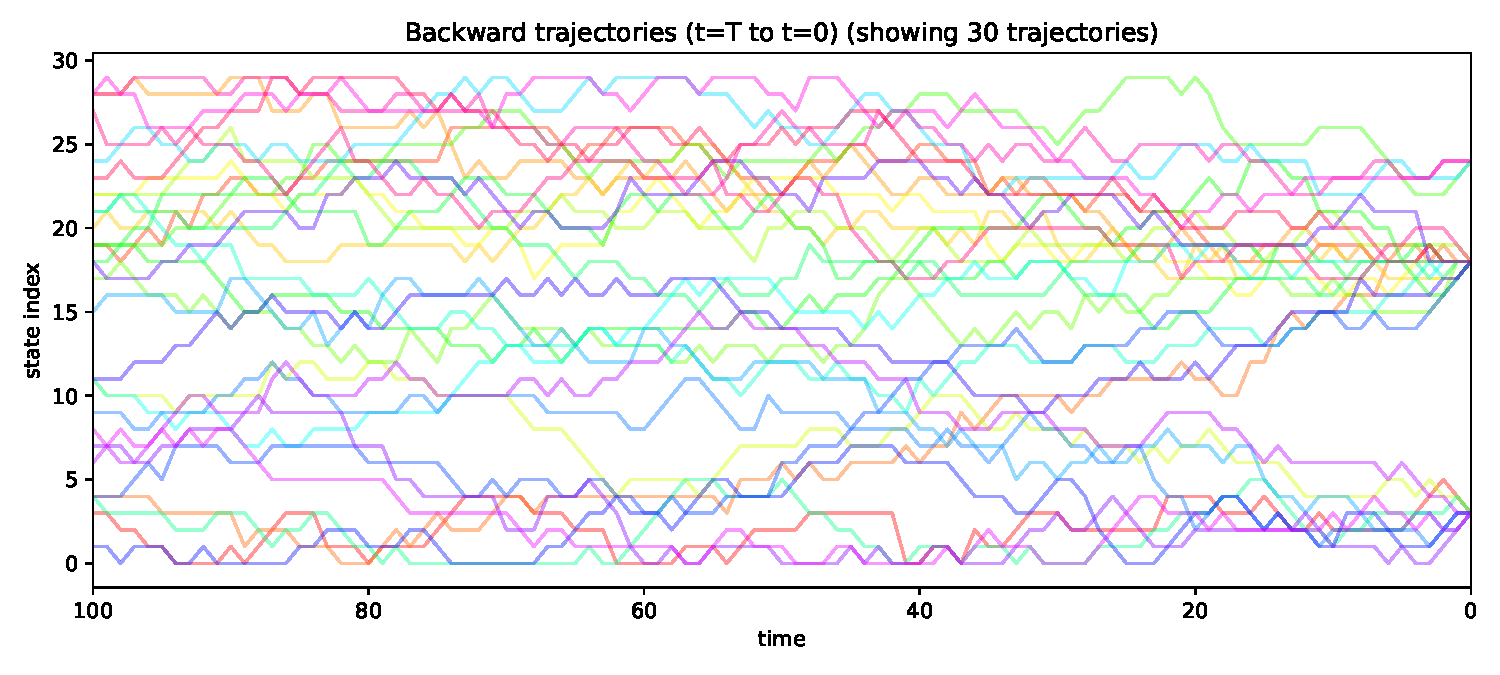
\includegraphics[width=\linewidth]{../tutorial/figures/backward_trajectories.pdf}
\end{column}
\begin{column}{0.49\textwidth}
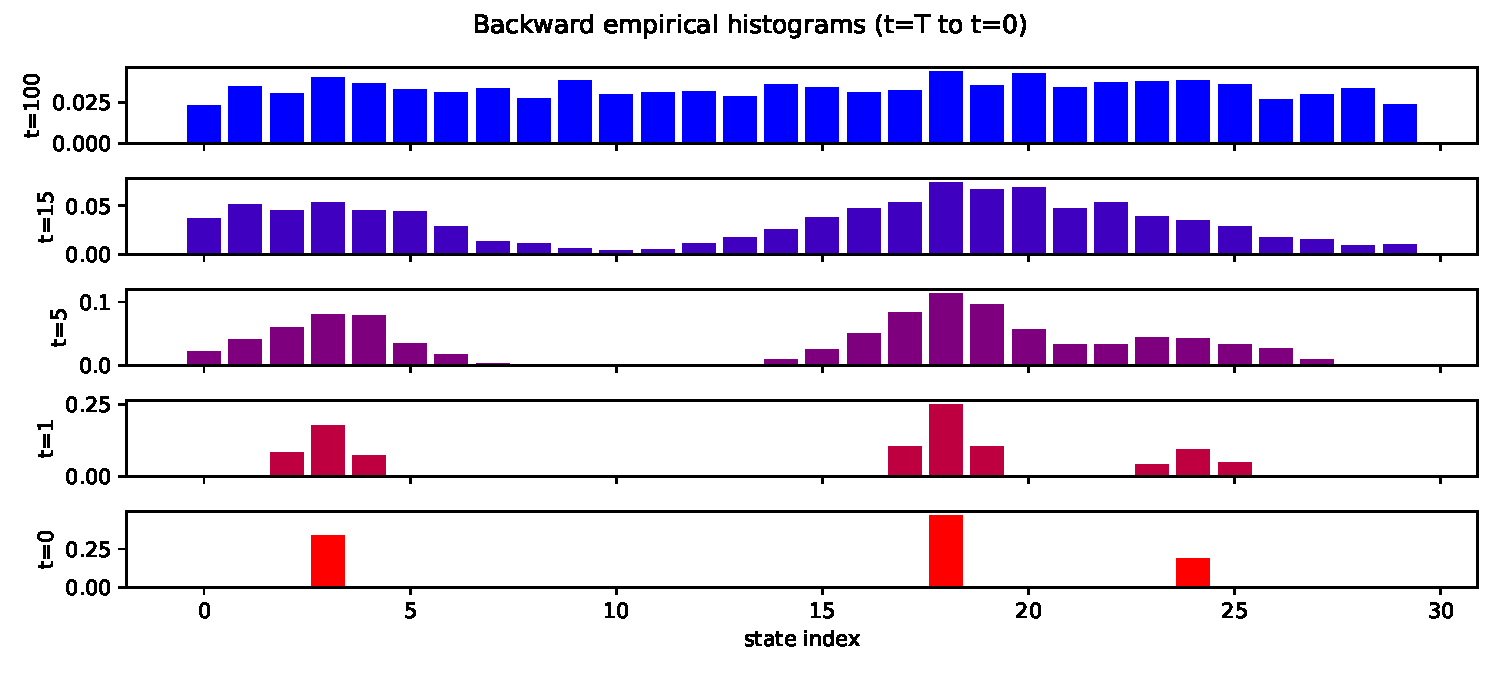
\includegraphics[width=\linewidth]{../tutorial/figures/backward_histograms.pdf}
\end{column}
\end{columns}
\vspace{0.4em}
\small Time is displayed from $T$ (left) to $0$ (right) in trajectories.
\end{frame}

\section{Learning Reverse Kernels}

\begin{frame}{Learning Objective}
From forward samples $(X_{t-1}^{(m)},X_t^{(m)},t_m)$, minimize
\[
\mathcal L(\theta)
=-\frac1M\sum_{m=1}^M
\log Q_\theta^{t_m-1}\big(X_{t_m}^{(m)},X_{t_m-1}^{(m)}\big).
\]

\begin{itemize}
\item This is cross-entropy on previous-state prediction.
\item Population form:
\[
\mathcal R(\theta)=C_\star+\mathbb E\big[\KL(Q_\star^t(i,\cdot)\|Q_\theta^t(i,\cdot))\big].
\]
\item Optional consistency regularization:
\[
\Delta(\theta)=\frac1T\sum_t\|(Q_\theta^t)^\top h^{t+1}-h^t\|_1.
\]
\end{itemize}
\end{frame}

\begin{frame}{Model Parameterization (Pedagogical)}
For 1D geometric histograms, encode
\[
x=\frac{i}{n-1}\in[0,1],\qquad \tau=\frac{t}{T}\in[0,1].
\]
Input is 2D: $(x,\tau)$ (not one-hot in geometric setting).

\begin{block}{2-layer MLP}
\[
(x,\tau)\xrightarrow{\text{Linear }(2\to p)}\mathrm{ReLU}\xrightarrow{\text{Linear }(p\to n)}\mathrm{Softmax}
\]
with $p=4n$.
\end{block}

If no spatial prior is available, replace $x$ by $\mathrm{onehot}(i)$.
\end{frame}

\begin{frame}[fragile]{Minimal Python Example}
\begin{lstlisting}[style=py]
class ReverseNet(nn.Module):
    def __init__(self, n, p):
        super().__init__()
        self.fc1 = nn.Linear(2, p)
        self.fc2 = nn.Linear(p, n)

    def forward(self, x_norm, t_norm):
        z = torch.cat([x_norm, t_norm], dim=1)
        z = F.relu(self.fc1(z))
        return torch.softmax(self.fc2(z), dim=1)

# x_norm = i/(n-1), t_norm = t/T
# loss = -log Q_theta^{t-1}(x_t, x_{t-1}) averaged over samples
\end{lstlisting}
\end{frame}

\section{Takeaways}

\begin{frame}{Takeaways and Practical Checklist}
\begin{itemize}
\item Forward recursion: $h^{t+1}=P^\top h^t$.
\item Reverse admissibility: $Q^t\in\Tset(h^{t+1},h^t)$.
\item Canonical inverse: Bayes kernel $Q^{\mathrm B,t}=\diag(h^{t+1})^+P^\top\diag(h^t)$.
\item Learning: optimize NLL on transitions; monitor marginal consistency.
\item Numerics: compare true vs learned $\log Q^t_{\lfloor n/2\rfloor,:}$ at multiple times.
\end{itemize}
\end{frame}

\end{document}
